% !TEX encoding = UTF-8 Unicode
\documentclass[a4paper]{article}


\usepackage{color}
\usepackage{url}
\usepackage[T2A]{fontenc} % enable Cyrillic fonts
\usepackage[utf8]{inputenc} % make weird characters work
\usepackage{graphicx}
\usepackage{here} 



\usepackage[english,serbian]{babel}
%\usepackage[english,serbianc]{babel} %ukljuciti babel sa ovim opcijama, umesto gornjim, ukoliko se koristi cirilica

\usepackage[unicode]{hyperref}
\hypersetup{colorlinks,citecolor=green,filecolor=green,linkcolor=blue,urlcolor=blue}

\usepackage{listings}

%\newtheorem{primer}{Пример}[section] %ćirilični primer
\newtheorem{primer}{Primer}[section]

\definecolor{mygreen}{rgb}{0,0.6,0}
\definecolor{mygray}{rgb}{0.5,0.5,0.5}
\definecolor{mymauve}{rgb}{0.58,0,0.82}

\lstset{ 
  backgroundcolor=\color{white},   % choose the background color; you must add \usepackage{color} or \usepackage{xcolor}; should come as last argument
  basicstyle=\scriptsize\ttfamily,        % the size of the fonts that are used for the code
  breakatwhitespace=false,         % sets if automatic breaks should only happen at whitespace
  breaklines=true,                 % sets automatic line breaking
  captionpos=b,                    % sets the caption-position to bottom
  commentstyle=\color{mygreen},    % comment style
  deletekeywords={...},            % if you want to delete keywords from the given language
  escapeinside={\%*}{*)},          % if you want to add LaTeX within your code
  extendedchars=true,              % lets you use non-ASCII characters; for 8-bits encodings only, does not work with UTF-8
  firstnumber=1000,                % start line enumeration with line 1000
  frame=single,	                   % adds a frame around the code
  keepspaces=true,                 % keeps spaces in text, useful for keeping indentation of code (possibly needs columns=flexible)
  keywordstyle=\color{blue},       % keyword style
  language=Python,                 % the language of the code
  morekeywords={*,...},            % if you want to add more keywords to the set
  numbers=left,                    % where to put the line-numbers; possible values are (none, left, right)
  numbersep=5pt,                   % how far the line-numbers are from the code
  numberstyle=\tiny\color{mygray}, % the style that is used for the line-numbers
  rulecolor=\color{black},         % if not set, the frame-color may be changed on line-breaks within not-black text (e.g. comments (green here))
  showspaces=false,                % show spaces everywhere adding particular underscores; it overrides 'showstringspaces'
  showstringspaces=false,          % underline spaces within strings only
  showtabs=false,                  % show tabs within strings adding particular underscores
  stepnumber=2,                    % the step between two line-numbers. If it's 1, each line will be numbered
  stringstyle=\color{mymauve},     % string literal style
  tabsize=2,	                   % sets default tabsize to 2 spaces
  title=\lstname                   % show the filename of files included with \lstinputlisting; also try caption instead of title
}

\begin{document}

\title{Informacioni sistem za firmu Duma Group\\ \small{Seminarski rad u okviru kursa\\Informacioni sistemi\\ Matematički fakultet}}

\author{Miloš Miković, Anđela Križan, Milica Galjak, \\ Veronika Miljaković, Nikoleta Vukajlović}

%\date{9.~april 2015.}

\maketitle

\abstract{
%Ovde ide abstract
}

\tableofcontents

\newpage

\section{Uvod}

 Sistem je skup delova koji funkcionišu zajedno radi ostvarenja zajedničkog cilja ili svrhe. U domenu informatike i računarstva značajnu ulogu imaju \textbf{Informacioni sistemi}. Internacionalna federacija za obradu podataka (International Federation for Information Processing - IFIP) definiše informacioni sistem na sljedeći način: "Informacioni sistem je sistem koji prikuplja, pohranjuje, čuva, obrađuje i isporučuje informacije važne za organizaciju i društvo, tako da budu dostupne i upotrebljive za svakog ko se želi njima koristiti, uključujući poslovodstvo, klijente, zaposlene i ostale. Informacioni sistem aktivni je društveni sistem koji se može, ali i ne mora, koristiti      informacionom tehnologijom." 
    
 Predmet ovog rada je razvijanje informacionog sistema za firmu Duma Group iz Novog Sada. Izrađen je kao grupni projekat u okviru predmeta Informacioni sistemi, koji se sluša na prvoj godini master studija Matematičkog fakulteta u Beogradu.

\section{Analiza sistema}

Firma Duma Group se bavi organizovanjem proslava i događaja. U firminoj ponudi nalaze se brojne usluge čiji je cilj da obezbedi korisnicima sve ono što im je za njihove događaje potrebno. Među ovim uslugama su ketering, fotograf, prenosivi bar, slatki sto...

Prilikom formiranja ovog informacionog sistema poseban akcenat ćemo staviti na mađusobnu komunikaciju zaposlenih u firmi, kao i na komunikaciju sa klijentima, jer je to od velikog značaja za unapređenje firme.
    
Korisnici se registruju na sajt nakon čega stupaju u kontakt sa menadžerima firme. Menadžer treba od korisnika da dobije informacije o događaju koji korisnik pravi kako bi mu predložio adekvatnu uslugu. Nakon toga menadžer prenosi osoblju korisnikove želje. 
Ukoliko se korisnik opredeli za usluge keteringa ili prenosivog bara, osoblje ima zadatak da pripremi sadržaj koji je korisnik tražio i zadovolji sve njegove potrebe. Dostavljači nakon toga dostavljaju korisniku sav sadržaj.
Ukoliko se korisnik opredeli za usluge fotografa dogovaraju se svi potrebni detalji nakon čega fotografi pripremaju potrebnu opremu za događaj. Na dan događaja odlaze na mesto održavanja gde fotografišu i snimaju korisnika i njegove goste. Nakon toga sledi izrada fotografija. 
    
Osnovna svrha sistema je da omogući korisnicima da njihov događaj izgleda onako kako su zamislili i da mu za njega budu dostupne sve usluge koje su im potrebne. 

Na slici \ref{fig:Tok} je prikazan dijagram toka podataka.
    
    \begin{figure}[H]
    \centering
    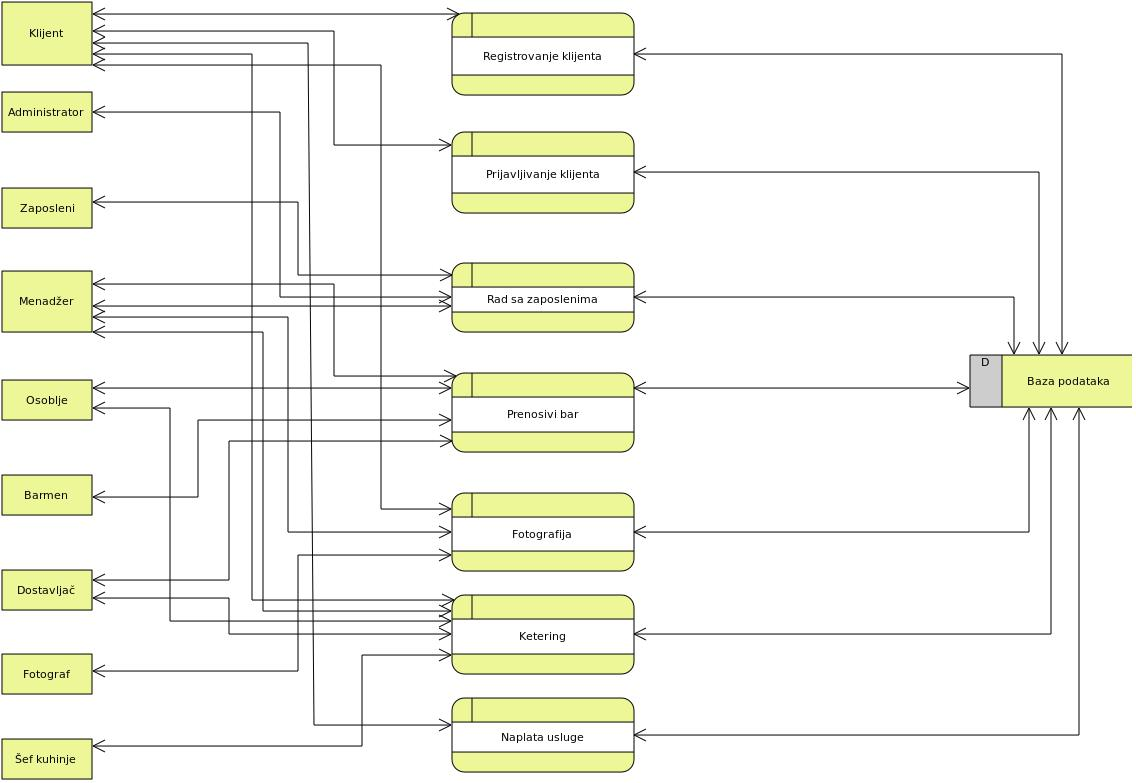
\includegraphics[width=14cm, height=14cm]{Nina/Data Flow Diagram1.jpg}
    \caption{Dijagram toka podataka}
    \label{fig:Tok}
\end{figure}
    
    \subsection{Učesnici u sistemu}
    
    \begin{enumerate}
        \item Klijent su svi oni kojima je potrebna usluga koju pruža firma Duma Group. Po završetku usluge vrše uplatu definisanih sredstava preko žiro računa.
        \item Menadžer je osoba koja je zadužena za komunikaciju između klijenta i zaposlenih. Prihvata ponudu i pristupa informacijama za kontaktiranje zaposlenih i klijenata putem informacionog sistema.
        \item Administrator je osoba koja je zadužena da obavi registraciju zaposlenog koji nema kreiran nalog u sistemu, kao i da obriše nalog nakon prekida radnog odnosa sa zaposlenim.
        \item Osoblje su svi oni koji su zaposleni za određeni događaj. Zadatke dobijaju od zaposlenih kao što je menadžer, šef kuhinje...
        \item Šef kuhinje je osoba koja je zadužena da upravlja organizacijom posla u kuhinji. Nadređeni je osoblju u kuhinji i zadužen je za podelu posla u kuhinji. Informacije o samom događaju prima od menadžera.
        \item Fotografi su osobe koje su zadužene za fotografisanje i snimanje gostiju na događaju. Nakon događaja njihov zadatak je da obrade materijal i pripreme finalni proizvod u vidu albuma ili buka. Informacije o događaju i zahtevima klijenta prima od menadžera.
        \item Barmen je osoba koja je zadužena za posluživanje pića gostima i beleženje toga šta je popijeno, u sklopu usluge Prenosivi bar
        \item Gosti su oni koji bivaju usluženi na događaju.
        \item Dostavljač je osoba koja je zadužena da isporuči poručenu opciju od strane klijenta. Detalje o samoj isporuci dobija putem aplikacije.
    \end{enumerate}
    
    
\section{Slučajevi upotrebe}

% Ovo je moj deo - Miloš

\subsection{Registrovanje i prijavljivanje korisnika}

\begin{figure}[htp]
    \centering
    
\includegraphics[width=8cm]{Miloš/Miloš_Slučajevi_upotrebe_slike/Slucaj upotrebe _Registrovanje.jpg}
    \caption{Dijagram slučaja upotrebe Registracija korisnika}
    \label{fig:Registracija}
\end{figure}

\subsubsection{Registrovanje klijenta}

\begin{itemize}
    \item Kratak opis:
        \begin{itemize}
            \item Klijent se registruje kako bi mogao da koristi mogućnosti informacionog sistema Duma Group
        \end{itemize}
    \item Učesnici:
        \begin{itemize}
            \item Klijent koji želi da koristi usluge Duma Group sistema
        \end{itemize}
    \item Preduslov:
        \begin{itemize}
            \item Klijent poseduje računar ili pametni telefon i pristup Internetu
            \item Sistem je u funkciji
        \end{itemize}
    \item Postuslov:
        \begin{itemize}
            \item Klijent je registrovan i otvoren mu je nalog za korišćenje sistema
        \end{itemize}
    \item Glavni tok:
        \begin{enumerate}
            \item  Klijent otvara stranicu za registraciju odabirom određenog dugmeta na sajtu sistema
            \item Klijent čita uslove korišćenja sistema i prihvata ih
            \item Klijent popunjava formular unoseći tražene lične podatke. Kada zavši popunjavanje formulara pritiska dugme za registraciju
            \item Sistem obrađuje podatke i vrši validaciju
            \item Sistem kreira privremeni korisnički nalog
            \item Sistem šalje klijentu poruku na e-mail adresu unetu u formularu, postavlja predviđeno vreme za aktivaciju naloga i čeka
            \item Klijent proverava poštu i potvrđuje link za registraciju
            \item Sistem obeležava korisnički nalog kao aktivan i čuva podatke o nalogu
            \item Sistem obaveštava klijenta slanjem poruke na e-mail adresu klijenta da je nalog uspešno kreiran 
        \end{enumerate}
    \item Alternativni tok:
        \begin{itemize}
            \item Prilikom 2. koraka glavnog toka klijent odbija uslove korišćenja sistema. Sistem obaveštava korisnika da mora da prihvati date uslove korišćenja, vraća ga na 2. korak glavnog toka i onemogućava dalji tok registracije dok klijent ne prihvati date uslove.
            \item Prilikom 4. koraka glavnog toka ukoliko klijent nije uneo ispravne podatke, sistem obaveštava klijenta i proces se nastavlja od 3. koraka glavnog toka
            \item Ukoliko klijent nije prihvatio aktivacionu poruku u 7. koraku glavnog toka u određenom vremenskom periodu, sistem briše nalog i proces se završava.
            \item Ukoliko u 7. koraku glavnog toka klijent nije primio aktivacionu poruku on obaveštava sistem da mu ponovo pošalje poruku i proces se nastavlja od koraka 6. glavnog toka
        \end{itemize}
    \item Dodatne informacije:
        \begin{itemize}
            \item Potrebni podaci za registraciju su korisničko ime, lozinka, potvrda lozinke, broj kreditne kartice, ime, prezime, e-mail naloga, e-mail za povratak naloga ako se desi da je korisnik zaboravi lozinku ili korisničko ime, datum rodjenja korisnika, pol korisnika
            \item Ova registracija predstavlja registraciju klijenata sistema, postoji i registracija zaposlenih koja se vrši odvojeno
        \end{itemize}
\end{itemize}

\begin{figure}[htp]
    \centering
    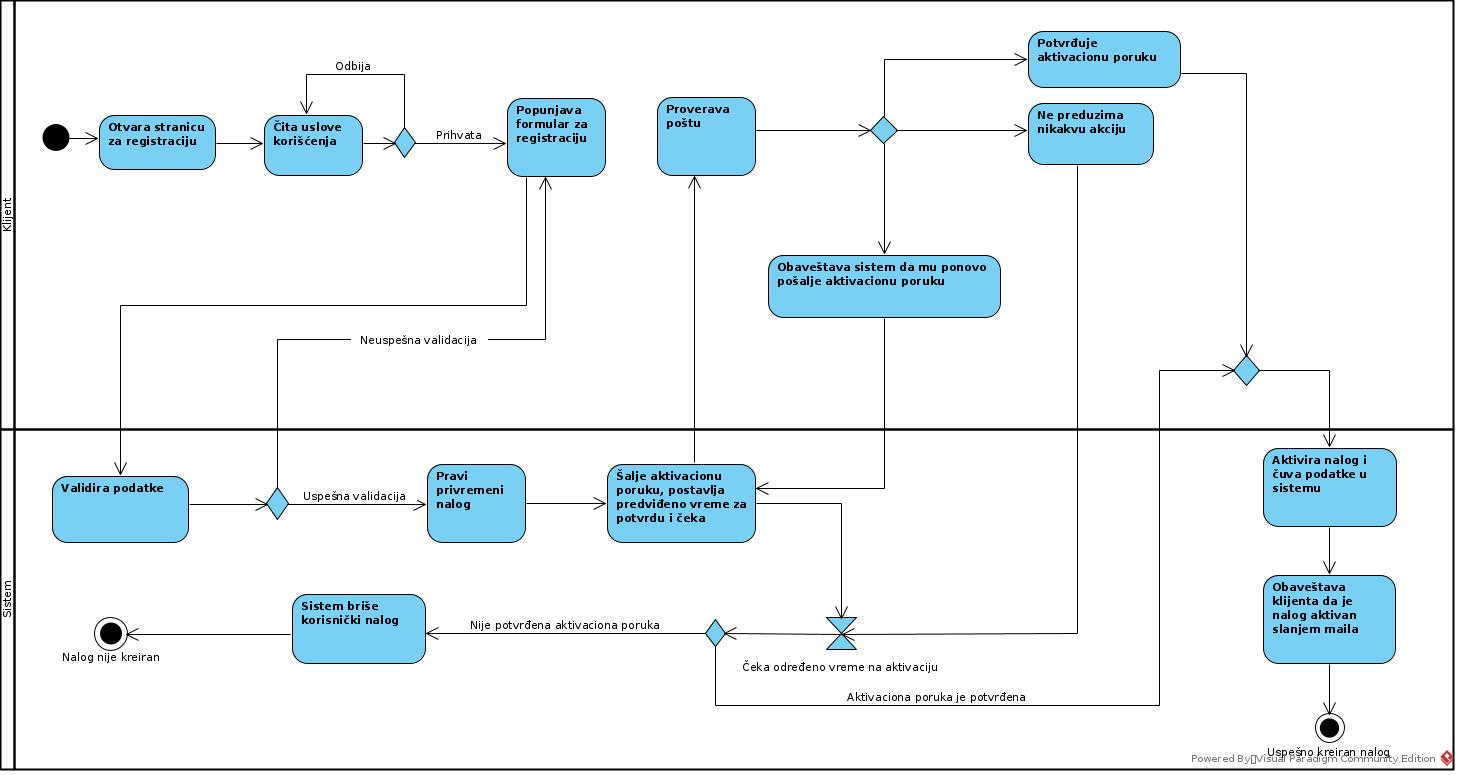
\includegraphics[width=10cm]{Miloš/Miloš_Dijagrami_aktivnosti_slike/Dijagram_aktivnosti_Registrovanje.jpg}
    \caption{Dijagram aktivnosti - Registrovanje korisnika}
    \label{fig:Registracija aktivnost}
\end{figure}


\subsubsection{Prijavljivanje korisnik}

\begin{figure}[htp]
    \centering
    
\includegraphics[width=8cm]{Miloš/Miloš_Slučajevi_upotrebe_slike/Slucaj upotrebe _Prijavljivanje.jpg}
    \caption{Dijagram slučaja upotrebe Prijavljivanje korisnika}
    \label{fig:Prijavljivanje}
\end{figure}

\begin{itemize}
    \item Kratak opis:
        \begin{itemize}
            \item Prethodno registrovani korisnik se prijavljuje na sistem
        \end{itemize}
    \item Učesnici:
        \begin{itemize}
            \item Registrovani korisnik koji želi da se prijavi na sistem
        \end{itemize}
    \item Preduslov:
        \begin{itemize}
            \item Korisnik mora biti registrovan u sistemu da bi se uspešno prijavio
            \item Korisnik poseduje računar ili pametni telefon i pristup Internetu
            \item Sistem je u funkciji
        \end{itemize}
    \item Postuslov:
        \begin{itemize}
            \item Korisnik je priavljen i može da koristi funkcionalnosti koje sistem pruža
        \end{itemize}
    \item Glavni tok:
        \begin{enumerate}
            %Možda da dodate početni korak da se otvara odgovarajuća stranica za
            %prijavu na sistem. Drugi korak može da se podeli na dva koraka. Sistem
            %proverava podatke i sistem prosleđuje korisnika dalje.
            \item Korisnik otvara stranicu za prijavljivanje
            \item Korisnik unosi svoje korisničko ime i šifru koju je koristio pri registraciji
            \item Sistem validira podatke
            \item Sistem sprovodi korisnika ka interfejsu aplikacije
        \end{enumerate}
    \item Alternativni tok:
        \begin{itemize}
            \item Ukoliko u 1. koraku glavnog toka korisnik ne može da se seti podataka za prijavljivanje obaveštava sistem da mu pošalje mail za oporavak. Sistem šalje mail korisniku, korisnik proverava mail i menja podatke u skladu sa instrukcijama koje je dobio u mailu. Sistem čuva izmene koje je korisnik napravio a proces se nastavlja od 1. koraka glavnog toka.
            \item Ukoliko u 3. koraku glavnog toka korisnički podaci nisu ispravni, sistem obaveštava korisnika o grešci i postavlja brojač neuspešnih pokušaja.
            Ako je brojač prethodno postavljen, njegova vrednost se uvećava za jedan. Proces se nastavlja od 2. koraka glavnog toka.
            \item Ukoliko sistem u 3. koraku glavnog toka određen broj puta ne uspe da validira korisničke podatke postavlja zabranu prijavljivanja za tog korisnika na određeni vremski period. Nakon isteka zabrane izvršavanje se nastavlja od 2. koraka glavnog toka.
        \end{itemize}
    \item Dodatne informacije:
        \begin{itemize}
            \item Zabrana prijavljivanja nakon nekoliko neuspešnih pokušaja postoji radi zaštite podataka i informacija sistema od eventualnih napada.
            \item Prijavljivanje se vrši na isti način i za klijente i za zaposlene u Duma Group preduzeću
        \end{itemize}
\end{itemize}


\begin{figure}[htp]
    \centering
    
\includegraphics[width=10cm]{Miloš/Miloš_Dijagrami_aktivnosti_slike/Dijagram_aktivnosti_Prijavljivanje.jpg}
    \caption{Dijagram aktivnosti - Prijavljivanje korisnika}
    \label{fig:Prijavljivanje aktivnost}
\end{figure}

%Ovo je moj deo - Veronika


\subsection{Prenosivi bar}

\begin{figure}[H]
    \centering
    \includegraphics[width=8cm]{Veronika/Dijagram slucaja upotrebe PB.jpg}
    \caption{Dijagram slučaja upotrebe Prenosivi bar}
    \label{fig:PrenosiviBar}
\end{figure}

\subsubsection{Odabir ponude}

\begin{itemize}
    \item Kratak opis:
        \begin{itemize}
            \item Klijent bira odgovarajuću ponudu u skladu sa događajem za koji mu je usluga potrebna
        \end{itemize}
    \item Učesnici:
        \begin{itemize}
            \item Klijent
            \item Menadžer za prenosivi bar
        \end{itemize}
    \item Preduslov:
        \begin{itemize}
            \item Klijent se prijavio u sistem
		    \item Na raspolaganju je spisak ponuda sa pratećim informacijama, slikama i snimcima
        \end{itemize}
    \item Postuslov:
        \begin{itemize}
            \item Klijent je odabrao odgovarajuću ponudu
            \item Menadžer je prihvatio odabir i zabeležio potrebne detalje u sistem
        \end{itemize}
    \item Glavni tok:
        \begin{enumerate}
		    \item Klijent se klikom na dugme opredeljuje za uslugu ''Prenosivi bar'' nakon čega sistem preusmerava klijenta na mejl menadžera za ovu uslugu
		    \item Klijent objašnjava menadžeru kog je tipa događaj i za šta mu je potreban bar
		    \item Menadžer mu na mejl šalje ponudu iz  sistema koja najviše odgovara tom tipu događaja, koja se sastoji od slika, snimaka i cene za konkretne sadržaje
		    \item Klijent bira sadržaj koji želi iz ponude i svaki odabir se beleži u sistem
		    \item Klijent dogovara sa menadzerom detalje o datumu događaja, njegovom trajanju, dodatnim zahtevima i upitima
		    \item Menadžer beleži sve dogovorene detalje u sistemu i rezerviše odgovarajući datum u sistemu
		    \item Menadžer u sistemu formira račun za klijenta na koji se dodaju cene prenosivog bara i dekoracije. Cene pića dodaju se naknadno jer klijent plaća samo ono što je na događaju popijeno.
        \end{enumerate}
    \item Alternativni tok:
        \begin{itemize}
            \item Korak 5 - Sadržaj koji je klijent odabrao nije dostupan. U tom slucaju menadžer zamoli klijenta da odabere nešto drugo iz ponude i uputi ga na ponudu koja je slična onoj koju je tražio. Nakon toga klijent ponovo bira sadržaj za svoj događaj.
        \end{itemize}
\end{itemize}


\begin{figure}[H]
    \centering
    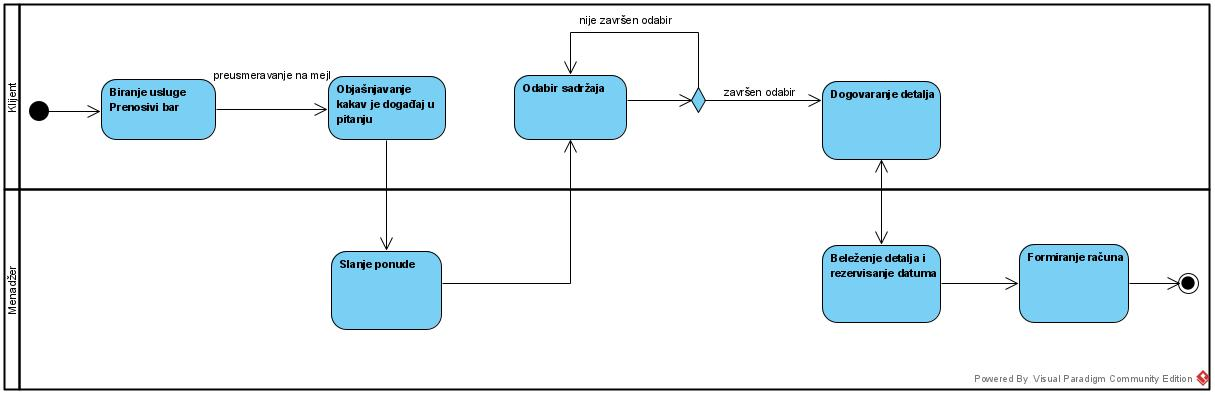
\includegraphics[width=8cm]{Veronika/Dijagram aktivnosti 1 PB.jpg}
    \caption{Dijagram aktivnosti - Odabir ponude}
    \label{fig:PrenosiviBar}
\end{figure}


\subsubsection{Priprema ponude}

\begin{itemize}
    \item Kratak opis:
        \begin{itemize}
            \item Menadžer za Prenosivi bar prenosi ponudu osoblju koje nakon toga priprema ono što je zahtevano
        \end{itemize}
    \item Učesnici:
        \begin{itemize}
            \item Menadžer za prenosivi bar
            \item Osoblje
        \end{itemize}
    \item Preduslov:
        \begin{itemize}
            \item Klijent je odabrao svoju ponudu
		    \item Menadžer za prenosivi bar je zabeležio ponudu u sistemu
        \end{itemize}
    \item Postuslov:
        \begin{itemize}
            \item Ponuda je pripremljena i spakovana za dostavu
        \end{itemize}
    \item Glavni tok:
        \begin{enumerate}
           \item Menadžer preko sistema šalje izabranu ponudu osoblju tako što odabere u sistemu sve one koji trebaju biti angažovani na događaju i na njihove naloge pošalje koja su im zaduženja
		   \item Osoblje preko svojih naloga preuzima detalje o ponudi
	       \item Osoblje proverava u sistemu da li je sve potrebno za događaj dostupno u magacinu i ako jeste priprema ono što je potrebno
	        \item Osoblje pakuje sav pripremljeni sadržaj u prevozno sredstvo tako da bezbedno stigne na dogovorenu lokaciju 
        \end{enumerate}
    \item Alternativni tok:
        \begin{itemize}
            \item Koraci 3 - Nešto od potrebnog sadržaja nije dostupno u magacinu. U tom slučaju zadatak menadžera je da zaduži nekog od osoblja da nabavi to što je neophodno.
        \end{itemize}
\end{itemize}

\begin{figure}[H]
    \centering
    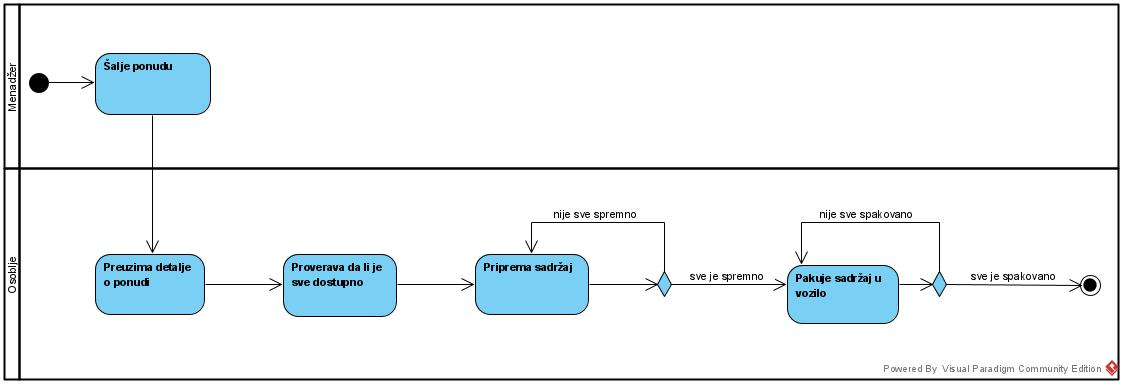
\includegraphics[width=8cm]{Veronika/Dijagram aktivnosti 2 PB.jpg}
    \caption{Dijagram aktivnosti - Priprema ponude}
    \label{fig:PrenosiviBar}
\end{figure}


\subsubsection{Dostava ponude}

\begin{itemize}
    \item Kratak opis:
        \begin{itemize}
            \item Ponuda je dovezena na potrebnu lokaciju i spremna za posluživanje
        \end{itemize}
    \item Učesnici:
        \begin{itemize}
            \item Dostavljač
            \item Osoblje
        \end{itemize}
    \item Preduslov:
        \begin{itemize}
            \item Sva potrebna roba je spakovana u prevozno sredstvo
		    \item Dostavljač je na raspolaganju	
        \end{itemize}
    \item Postuslov:
        \begin{itemize}
            \item Sve je postavljeno po dogovoru i spremno za početak događaja
        \end{itemize}
    \item Glavni tok:
        \begin{enumerate}
            \item Dostavljač preuzima informaciju iz sistema gde treba odvesti porudžbinu i osoblje zaduženo za postavljanje
           \item Dostavljač odvozi robu i osoblje na dogovorenu adresu sat vremena pre početka događaja 
		    \item Osoblje montira prenosivi bar i dekoriše ga onako kako je u sistemu zabeleženo da je korisnik zahtevao
        \end{enumerate}
    
\end{itemize}

\begin{figure}[H]
    \centering
    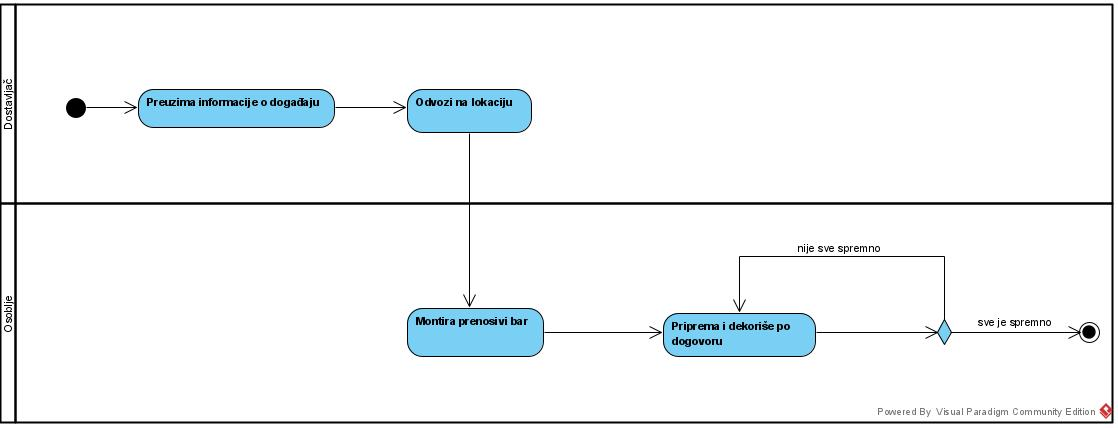
\includegraphics[width=8cm]{Veronika/Dijagram aktivnosti 3 PB.jpg}
    \caption{Dijagram aktivnosti - Dostava ponude}
    \label{fig:PrenosiviBar}
\end{figure}

\subsubsection{Posluživanje gostiju}

\begin{itemize}
    \item Kratak opis:
        \begin{itemize}
            \item Gosti dolaze do šanka gde im barmen sipa pića i pravi odgovarajuće koktele 
        \end{itemize}
    \item Učesnici:
        \begin{itemize}
            \item Gosti
            \item Barmen
        \end{itemize}
    \item Preduslov:
        \begin{itemize}
            \item Barmen je dobio detalje o mestu i vremenu održavanja događaja
            \item Dostavljač je dovezao na događaj sve ono što je barmenu potrebno za pripremanje pića
        \end{itemize}
    \item Postuslov:
        \begin{itemize}
            \item Svi gosti su usluženi na odgovarajući način
            \item Na račun su dodate cene popijenih pića
        \end{itemize}
    \item Glavni tok:
        \begin{enumerate}
            \item Barmen dolazi na odgovarajuću adresu koja mu je poslata preko sistema i priprema se za posao
            \item Barmen iz sistema čita spisak pića koje je klijent naručio i proverava da li mu je dostavljeno sve što je naručeno
           \item Gost dolazi do šanka i naručuje piće od barmena
		   \item Barmen uslužuje gosta i beleži u sistem koje je piće naručeno
		   \item Sistem dodaje cenu tog pića na račun korisnika
		  \end{enumerate}
		\textit{Koraci 3,4,5 se ponavljaju za svakog gosta koji priđe šanku sve do kraja događaja}
	
    \item Alternativni tok:
        \begin{itemize}
	      \item	Korak 5 - Piće koje gost traži je u međuvremenu popijeno. U tom slučaju barmen preporučuje gostu neka druga pića koja su dostupna i gost bira jedno od njih.

        \end{itemize}
\end{itemize}

\begin{figure}[H]
    \centering
    \includegraphics[width=8cm]{Veronika/Dijagram aktivnosti 4 PB.jpg}
    \caption{Dijagram aktivnosti - Posluživanje gostiju}
    \label{fig:PrenosiviBar}
\end{figure}

\subsection{Rad sa zaposlenima}

\begin{figure}[H]
    \centering
    \includegraphics[width=8cm]{Nina/Slucaj upotrebe rad sa zaposlenima.jpg}
    \caption{Dijagram slučaja upotrebe Rad sa zaposlenima}
    \label{fig:RegistracijaZ}
\end{figure}

\subsubsection{Registracija zaposlenog}

\begin{itemize}
    \item Kratak opis: 
    \begin{itemize}
        \item Administrator registruje zaposlenog koji nema otvoren nalog u sistem Douma Group. Sistem izvršava validaciju i vraća potvrdu o registraciji, ukoliko je uspešna.
    \end{itemize}
    \item Učesnici:
        \begin{itemize}
        \item Administrator
        \item Zaposleni
    \end{itemize}
    \item Preduslovi:
        \begin{itemize}
            \item Zaposleni nema kreiran nalog.
            \item Sistem je u funkciji.
        \end{itemize}
    \item Postuslovi:
        \begin{itemize}
            \item Zaposleni je registrovan u sistem i dobija informacije kako da ga koristi.
        \end{itemize}
    \item Glavni tok:
        \begin{enumerate}
            \item Zaposleni popunjava obrazac sa potrebnim podacima za registraciju.
            \item Zaposleni predaje obrazac administratoru.
            \item Administrator proverava da li su podaci validni.
            \item Administrator popunjava formular sa podacima koje je dobio.
            \item Administrator bira poziciju zaposlenog.
            \item Sistem šalje obaveštenje administratoru da potvrdi unos.
            \item Administrator potvrđuje podatke klikom na dugme.
            \item Sistem obaveštava administratora da je uspešno registrovan nalog.
            \item Administrator šalje zaposlenom uputstvo za korišćenje sistema.
        \end{enumerate}
    \item Alternativni tokovi:
        \begin{itemize}
            \item Korak 3 - Ukoliko je obrazac nepravilno popunjen (nedostaju neki podaci), administrator obaveštava zaposlenog gde je napravljena greška kako bi je ispravio. Proces se nastavlja u koraku 1.
        \end{itemize}
\end{itemize}

\begin{figure}[H]
    \centering
    \includegraphics[width=10cm]{Nina/DijagramAktivnostiRegistracijaZaposlenog.jpg}
    \caption{Dijagram aktivnosti registracije zaposlenog}
    \label{fig:RegistracijaZ}
\end{figure}


\subsubsection{Brisanje naloga zaposlenog}

\begin{itemize}
    \item Kratak opis: 
    \begin{itemize}
        \item Briše se nalog zaposlenog sa kojim je prekinut radni odnos.
    \end{itemize}
    \item Učesnici:
        \begin{itemize}
        \item Menadžer za ketering/fotografiju/prenosivi bar
        \item Administrator
    \end{itemize}
    \item Preduslovi:
        \begin{itemize}
            \item Sa zaposlenim je prekinut radni odnos.
            \item Sistem je u funkciji.
        \end{itemize}
    \item Postuslovi:
        \begin{itemize}
            \item Nalog je obrisan.
        \end{itemize}
    \item Glavni tok:
        \begin{enumerate}
            \item Menadžer šalje zahtev administratoru da obriše nalog.
            \item Administrator pokreće postupak brisanja naloga zaposlenog klikom na dugme za brisanje.
            \item Administrator popunjava informacije o tome da li je zaposleni svojevoljno dao otkaz ili ne.
            \item Administrator potvrđuje brisanje.
            \item Sistem potvrđuje nalog kao obrisan.
        \end{enumerate}
\end{itemize}

\begin{figure}[H]
    \centering
    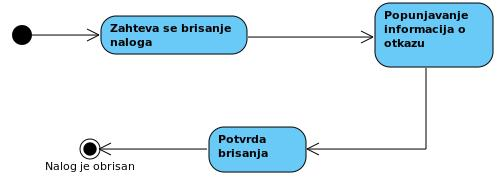
\includegraphics[width=8cm]{Nina/Dijagram_aktivnosti_brisanje_naloga.jpg}
    \caption{Dijagram aktivnosti brisanja naloga}
    \label{fig:RegistracijaZ}
\end{figure}

%%%%%%%%%%%%%%%%%%%%%%%%%%%%%%%%%%%%%%%%%%%%%%%%%%%%%%%%%%%%%%%%%%%%%%%%%%%%%%
% Ovo je moj deo - Andjela

\subsection{Fotografija}

\begin{figure}[htp]
    \centering
    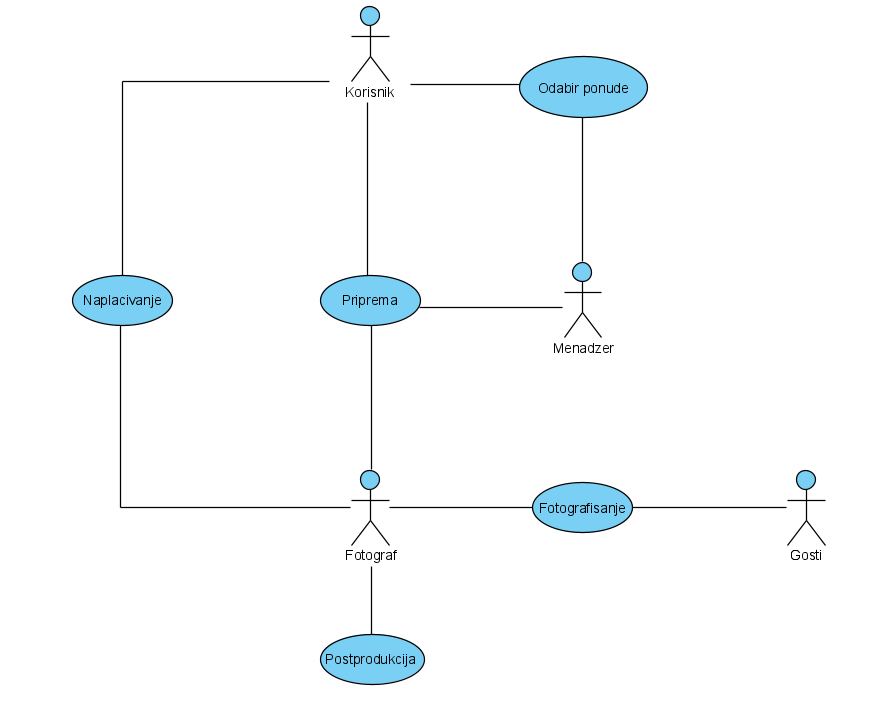
\includegraphics[width=8cm]{Andjela/fotografija_dijagram1.png}
    \caption{Dijagram slučaja upotrebe Fotografija}
    \label{fig:PrenosiviBar}
\end{figure}

\subsubsection{Odabir ponude}
\begin{itemize}
    \item Kratak opis: 
    \begin{itemize}
        \item Klijent bira odgovarajuću ponudu u skladu sa događajem za koji mu je usluga potrebna
    \end{itemize}
    \item Učesnici:
        \begin{itemize}
        \item Klijent
        \item Menadžer za fotografiju
    \end{itemize}
    \item Preduslovi:
        \begin{itemize}
            \item Klijent se registrovao na sajt
            \item Na raspolaganju je spisak ponuda različitih sa pratećim slikama i snimcima
        \end{itemize}
    \item Postuslovi:
        \begin{itemize}
            \item Klijent je odabrao odgovarajuću ponudu
            \item Menadžer je prihvatio izbor i zabeležio potrebne detalje u sistem
        \end{itemize}
    \item Glavni tok:
        \begin{enumerate}
            \item Klijent se ulogovao na sajt
            \item Klijent se opredeljuje za uslugu ''Fotografija'', nakon čega sistem preusmerava klijenta na mejl menadžera za ovu uslugu
            \item Klijent objašnjava menadžeru kog je tipa događaj i kakve fotografe želi
            \item Menadžer mu preko sistema šalje ponudu iz ''Fotografije'' sa pratećim informacijama o ceni i finalnom proizvodu 
            \item Klijent bira sadržaj iz ponude i to se beleži u sistem 
            \item Klijent se dogovara sa menadžerom oko detalja dogadaja (datum događaja, trajanje, dodatni zahtevi)
            \item Menadžer beleži sve dogovorene detalje u sistem i rezerviše odgovarajući datum u sistemu
            \item Menadžer u sistemu formira račun za klijenta na koji se dodaje cena fotografisanja i izrada finalnog proizvoda(foto album, buk, video snimak...)
        \end{enumerate}
        
    \begin{figure}[H]
    \centering
    \includegraphics[width=8cm]{Andjela/odabir_ponude_fotografija.png}
    \caption{Dijagram aktivnosti odabira ponude}
    \label{fig:RegistracijaZ}
\end{figure}
        
\end{itemize}

\subsubsection{Priprema}
\begin{itemize}
    \item Kratak opis: 
    \begin{itemize}
        \item Menadžer za Fotografiju obaveštava fotografe o rasporedu svečanosti
        %\item Klijent obaveštava o dodatnim zahtevima
    \end{itemize}
    \item Učesnici:
        \begin{itemize}
        %\item Klijent
        \item Fotografi
        \item Menadžer za Fotografiju
    \end{itemize}
    \item Preduslovi:
        \begin{itemize}
            \item Klijent je izabrao ponudu
            \item Menadžer za Fotografiju je prihvatio ponudu i zabeležio u sistem
        \end{itemize}
    \item Postuslovi:
        \begin{itemize}
            \item Fotografi su pripremili opremu u odnosu na zahtev
        \end{itemize}
    \item Glavni tok:
        \begin{enumerate}
            \item Menadžer preko sistema obaveštava fotografe o rasporedu svečanosti i zahtevima klijenta
            \item Fotografi preuzimaju detalje o zahtevima klijenta
            \item Fotografi pripremaju opremu (rasvetu, kameru, dron...)
            \item Fotografi pripremaju plan fotografisanja u skladu sa zahtevima korisnika
            \item Na dan proslave, fotografi setuju opremu
        \end{enumerate}
        
        \begin{figure}[H]
    \centering
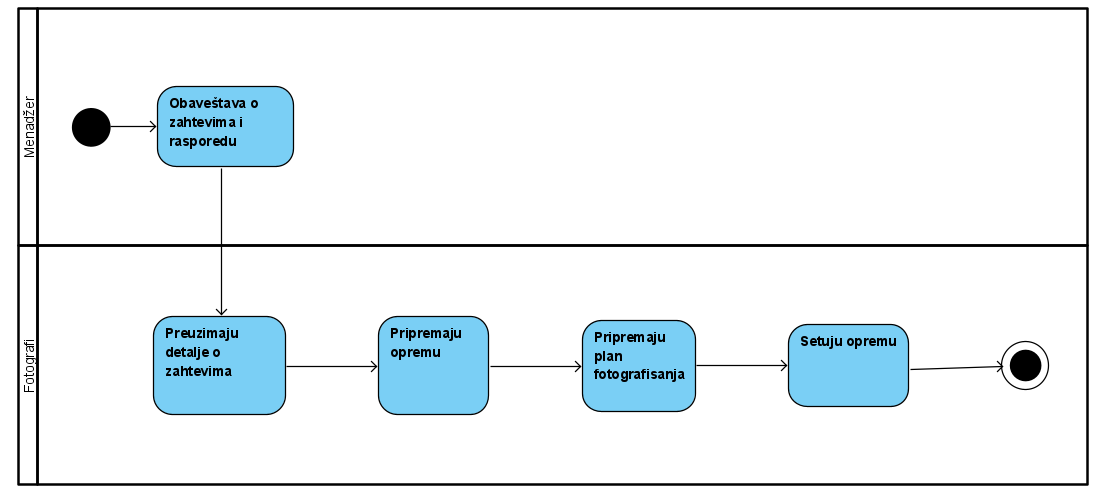
\includegraphics[width=8cm]{Andjela/priprema_fotografija.png}
    \caption{Dijagram aktivnosti pripreme}
    \label{fig:RegistracijaZ}
\end{figure}
        
        
\end{itemize}
\subsubsection{Fotografisanje}
\begin{itemize}
    \item Kratak opis: 
    \begin{itemize}
        \item Fotografi snimaju, fotografišu i menjaju pozicije kako bi zabeležili najvažnije trenutke
    \end{itemize}
    \item Učesnici:
        \begin{itemize}
        \item Gosti
        \item Fotografi
    \end{itemize}
    \item Preduslovi:
        \begin{itemize}
            \item Fotografi su dobili detalje o mestu i vremenu održavanja događaja
            \item Oprema je setovana
            \item Fotografi su na pozicijama i čekaju da svečanost počne
        \end{itemize}
    \item Postuslov:
        \begin{itemize}
            \item Snimljen je sirovi materijal
            \end{itemize}
    \item Glavni tok:
        \begin{enumerate}
            \item Fotografi dolaze na odgovarajuću adresu koja im je poslata preko sistema
            \item Snimanje i fotografisanje slavlja sa gostima
            \item Fotografisanje slavljenika
            
            \textit{Koraci 2 i 3 se ponavljaju za svakog gosta ili slavljenika koji želi da se fotogafiše tokom celog događaja}
        \end{enumerate}
    \item Alternativni tok:
        \begin{itemize}
            \item Korak 3 - Ukoliko je u pitanju svadba (Post Wedding), dan nakog proslave mladenci i fotografi idu na dogovorenu destinaciju radi fotografisanja
    \end{itemize}
    
    \begin{figure}[H]
    \centering
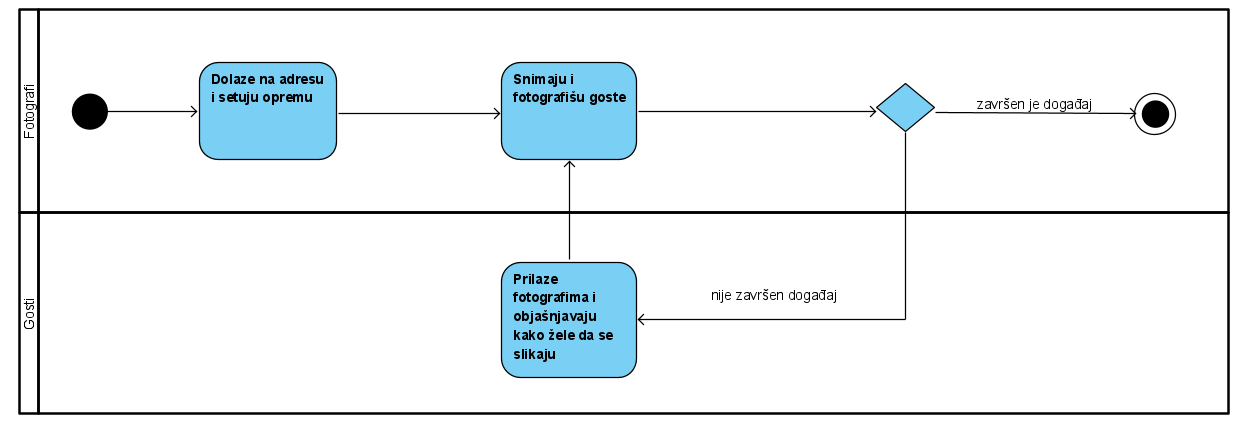
\includegraphics[width=8cm]{Andjela/fotografisanje.png}
    \caption{Dijagram aktivnosti fotografisanja}
    \label{fig:RegistracijaZ}
\end{figure}
    
        
\end{itemize}
\subsubsection{Postprodukcija}
\begin{itemize}
    \item Kratak opis: 
    \begin{itemize}
        \item Pregled i obrada sirovog materijala 
    \end{itemize}
    \item Učesnici:
        \begin{itemize}
        \item Fotografi
    \end{itemize}
    \item Preduslov:
        \begin{itemize}
            \item Sakupljen je sav sirovi materijal spreman za obradu
        \end{itemize}
    \item Postuslov:
        \begin{itemize}
            \item Gotov je konačni proizvod
            \end{itemize}
    \item Glavni tok:
        \begin{enumerate}
            \item Pregled sirovog materijala
            \item Izrada finalnog proizvoda od sakupljenih fotografija. Finalni proizvod može biti fotoalbum, fotografije u elektronskoj formi, buk
            \item Izrada finalnog proizvoda od sakupljenih video snimaka. Izbor najuspešnijih kadrova. Finalni proizvod može biti spot(od 30s do 180s), film (kraća i duža verzija)
            \textit{Koraci 2 i 3 se ponavljaju sve dok ne bude zavrsena obrada sirovog materijala i spreman finalni proizvod}
        \end{enumerate}
        
        \begin{figure}[H]
    \centering
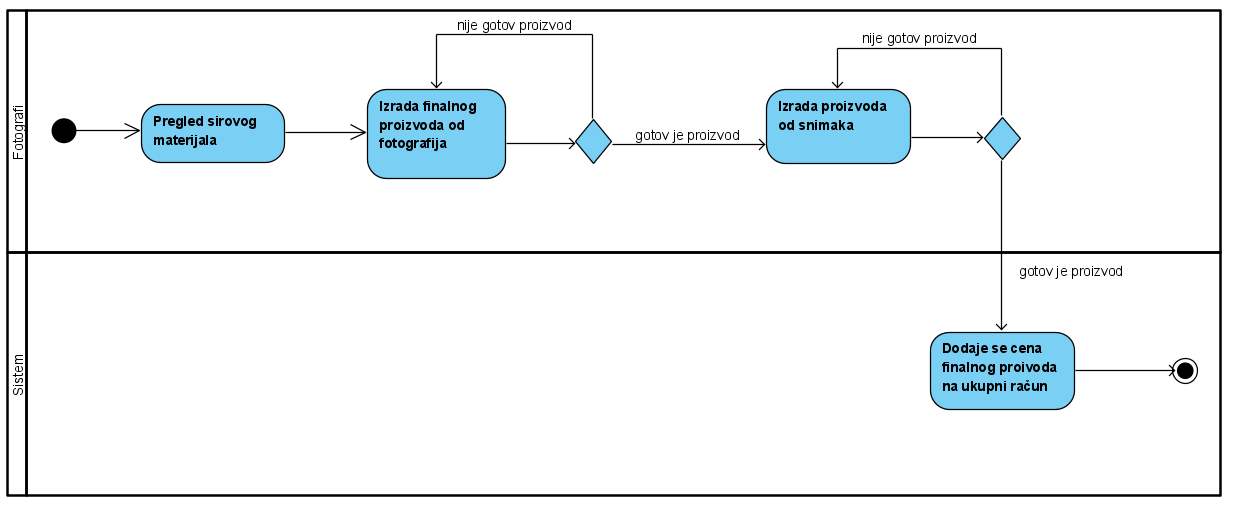
\includegraphics[width=8cm]{Andjela/postprodukcija.png}
    \caption{Dijagram aktivnosti postprodukcije}
    \label{fig:RegistracijaZ}
\end{figure}
        
        
\end{itemize}
% kraj-Andjela
%%%%%%%%%%%%%%%%%%%%%%%%%%%%%%%%%%%%%%%%%%%%%%%%%%%%%%%%%%%%%%%%%%%%%%%%%%%%%%


%%%%%%%%%%%%%%%%
%pocetak-Milica

\subsection{Ketering}

  
\begin{figure}[H]
\centering
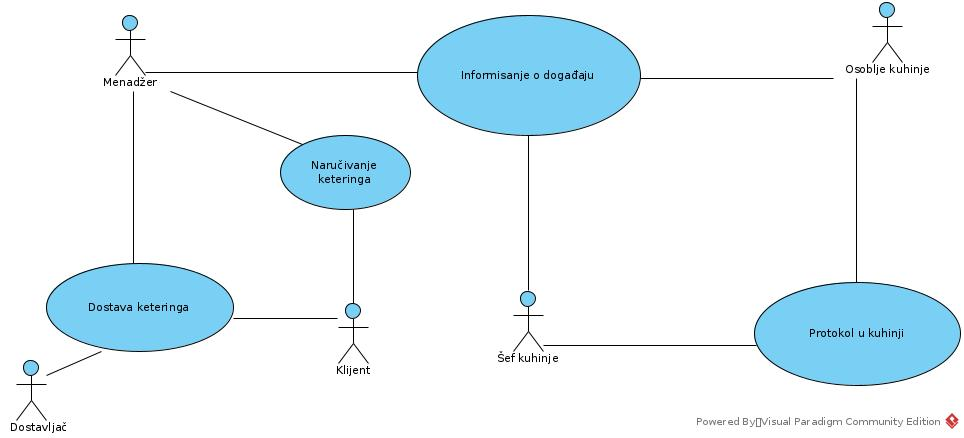
\includegraphics[width=13cm, height=6cm]{Milica/Ketering_Slucaj_upotrebe1.jpg}
\caption{Dijagram slučaja upotrebe Ketering}
\label{fig:Ketering}
\end{figure}

\subsubsection{Noručivanje keteringa i prihvatanje ponude}
\begin{itemize}
    \item Kratak opis:
    \begin{itemize}
 
        \item Klijent putem aplikacije bira željenu ponudu. Menadžer putem aplikacije dobija traženu ponudu, odnosno prihvata je.
    \end{itemize}
    
    
\end{itemize}


  \begin{itemize}
        \item Učesnici:
         \begin{itemize}
        \item Menadžer
    \end{itemize}
          \begin{itemize}
        \item Klijent
    \end{itemize}
    
    \end{itemize}
      \begin{itemize}
        \item Preduslov:
          \begin{itemize}
        \item Klijent je registrovan u sistemu.
       
   \end{itemize}
    
    \end{itemize}
      \begin{itemize}
        \item Postuslov:
          \begin{itemize}
        \item Porudžbina je naručena i prihvaćena od strane menadžera.
    \end{itemize}
    \end{itemize}
      \begin{itemize}
        \item Glavni tok:
          \begin{enumerate}
          
              \item Klijent, se uloguje na svoj nalog u aplikaciji, bira kao željenu opciju ketering.
              
              \item Zatim bira datum i vreme početka događaja za koji naručuje ketering i mesto.
          
              \item Nakon toga, bira iz asortimana na aplikaciji željenu ponudu i količinu.
              
              \item Potvrđuje izabranu porudžbinu.
        
              \item Menadžeru stiže obaveštenje od aplikacije da ima novu porudžbinu keteringa.
         
              \item Prihvata porudžbinu.
      
          \end{enumerate}
    \end{itemize}
    
   
    
\begin{figure}[H]
    \centering
    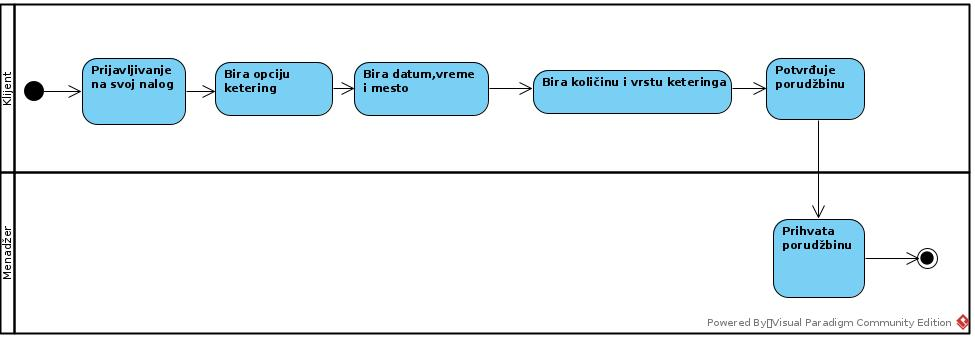
\includegraphics[width=15cm, height=5cm]{Milica/Dijagram_aktivnosti_Narucivanje.jpg}
    \caption{Dijagram aktivnosti Naručivanje keteringa i prihvatanje ponude}
    \label{fig:RegistracijaZ}
\end{figure}

    


\subsubsection{Formiranje tima za događaj}
\begin{itemize}
    \item Kratak opis:
    \begin{itemize}
        \item 
        Menadžer prihvata narudžbinu putem aplikacije. U zavisnosti od datuma za koji je naručena narudžbina, šalje zahtev osoblju koje je raspoloživo tada. Osoblje obeležava u aplikaciji da li želi da radi za zakazani događaj ili ne.
    \end{itemize}
\end{itemize}
  \begin{itemize}
        \item Učesnici:
          \begin{itemize}
        \item Menadžer
    \end{itemize}
      \begin{itemize}
        \item Osoblje
    \end{itemize}
    \begin{itemize}
        \item Šef kuhinje
    \end{itemize}
    \end{itemize}
      \begin{itemize}
        \item Preduslov:
          \begin{itemize}
        \item  Klijent je izabrao željenu ponudu korišćenjem aplikacije.
    \end{itemize}
    
    \end{itemize}
      \begin{itemize}
        \item Postuslov:
          \begin{itemize}
        \item Izabran je tim koji će raditi za zakazani događaj. Šef kuhinje zna koje osoblje je u timu.
    \end{itemize}
    \end{itemize}
      \begin{itemize}
        \item Glavni tok:
          \begin{enumerate}
              \item Menadžer šalje zahtev za potvrdu o radu raspoloživom osoblju. Sa zahtevom šalje i informacije o tipu događaja, detalje o samoj narudžbini keteringa.
        
              \item Svako od osoblja koje je dobilo zahtev vraća odgovor da li želi da radi narudžbinu ili ne.
         
        
              \item Menadžer ima spisak osoblja koje žele da rade događaj.
          
              \item Menadžer šalje spisak osoblja šefu kuhinje.
          \end{enumerate}
    \end{itemize}
      \begin{itemize}
        \item Alternativni tok:
          \begin{itemize}
        \item -Korak 4.-Ukoliko nema dovoljno osoblja za zakazani događaj, menadžer stupa u kontakt sa klijentom pomoću podataka koje je klijent osavio na svom nalogu na aplikaciji, obaveštava ga o tome i izlaže mu druge opcije kao što su promena termina događaja, manja količina poručene hrane...Ukoliko klijent prihvati druge opcije, menadžer ponovo sastavlja tim u skladu sa klijentovom željom da li želi drugi datum ili drugu porudžbinu. Proces se nastavlja u koraku 4.
    \end{itemize}
    \end{itemize}
    
    
\begin{figure}[H]
    \centering
    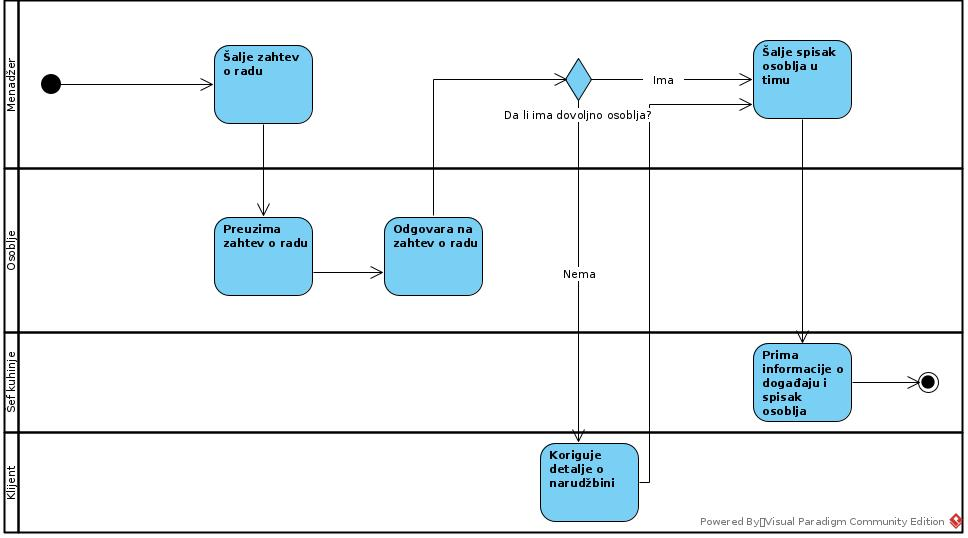
\includegraphics[width=13cm, height=8cm]{Milica/Dijagram_aktivnosti_Formiranje_tima.jpg}
    \caption{Dijagram aktivnosti Formiranje tima za događaj }
    \label{fig:FormiranjeTima}
\end{figure}

\subsubsection{Priprema hrane za događaj}
\begin{itemize}
    \item Kratak opis:
    \begin{itemize}
        \item Šef kuhinje zadaje zadatke za osoblje. Priprema hrane.
    \end{itemize}
\end{itemize}
  \begin{itemize}
        \item Učesnici:
          \begin{itemize}
        \item Šef kuhinje
    \end{itemize}
      \begin{itemize}
        \item Osoblje
    \end{itemize}
    \end{itemize}
      \begin{itemize}
        \item Preduslov:
          \begin{itemize}
        \item Šef kuhinje je obavešten o detaljima narudžbine. Šef kuhinje ima spisak osoblja koji su raspoloživi za događaj.
   \end{itemize}
    
    \end{itemize}
      \begin{itemize}
        \item Postuslov:
          \begin{itemize}
        \item Narudžbina je gotova za dogovoreno vreme.
    \end{itemize}
    \end{itemize}
      \begin{itemize}
        \item Glavni tok:
          \begin{enumerate}
              
        
              \item U zavisnosti od vrste hrane koja je naručena i sposobnostima osoblja, podeljeni su zadaci osoblju od strane šefa kuhinje. Svako od osoblja ima na aplikaciji koji je njegov deo posla, kao i koji su delovi posla ostalih članova u timu. 
        
              \item Svako od osoblja procenjuje koliko vremena je potrebno da izvrši zadati posao i  unosi procenjeno vreme u aplikaciju.
         
              \item U zavisnosti od procenjenog vremena osoblja i zakazanog termina dogadjaja, šef kuhinje zakazuje početak radnog vremena.
       
              \item U dogovoreno vreme, svako od osoblja počinje sa izvršavanjem svog dela posla.
          
              \item Ketering je spreman za dostavljanje.
          \end{enumerate}
    \end{itemize}
      \begin{itemize}
        \item Alternativni tok:
          \begin{itemize}
        \item -Korak 3.- Ukoliko procenjeno vreme završavanja posla prekorači zakazano vreme događaja, šef kuhinje šalje zahtev osoblju koje je odbilo zahtev menadžera a bilo je raspoloživo za datum događaja. Proces se nastavlja u koraku 3.
    \end{itemize}
    \end{itemize}
    
\begin{figure}[H]
    \centering
    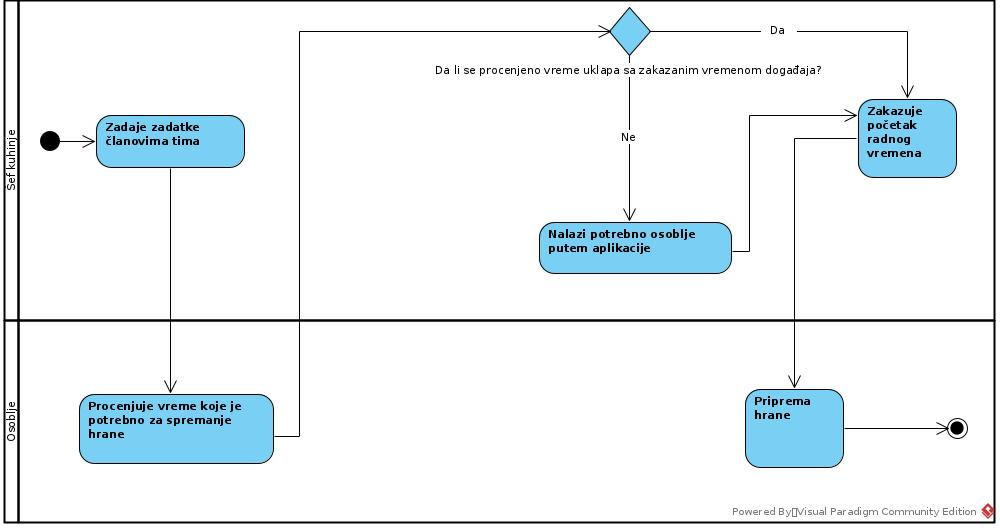
\includegraphics[width=14cm, height=8cm]{Milica/Dijagarm_aktivnosti_Priprema_hrane.jpg}
    \caption{Dijagram aktivnosti Priprema hrane }
    \label{fig:RegistracijaZ}
\end{figure}
    

\subsubsection{Dostava keteringa}
\begin{itemize}
    \item Kratak opis:
    \begin{itemize}
 
        \item Menadžer korišćenjem informacionog sistema obaveštava dostavljača o terminu i lokaciji isporuke poručenog keteringa. Dostavljač potvrđuje dostavu.Dostavljač prevozi u određeno vreme na određenu lokaciju poručeni ketering.
        Klijent preuzima ketering.
    \end{itemize}
    
    
\end{itemize}


  \begin{itemize}
        \item Učesnici:
         \begin{itemize}
        \item Menadžer:
    \end{itemize}
          \begin{itemize}
        \item Klijent:
    \end{itemize}
      \begin{itemize}
        \item Dostavljač:
    \end{itemize}
    \end{itemize}
      \begin{itemize}
        \item Preduslov:
          \begin{itemize}
        \item Osoblje u kuhinji je završilo posao na vreme.
       
   \end{itemize}
    
    \end{itemize}
      \begin{itemize}
        \item Postuslov:
          \begin{itemize}
        \item Porudžbina je dostavljena klijentu za događaj.
    \end{itemize}
    \end{itemize}
      \begin{itemize}
        \item Glavni tok:
          \begin{enumerate}
          
              \item Menadžer šalje zahtev dostavljaču preko aplikacije sa detaljima isporuke.
          
              \item Dostavljač potvrđuje da li je slobodan da dostavi porudžbinu ili ne.
              
              \item Dostavljač se informiše kako može da dođe na lokaciju događaja.Dostavljač uzima u obzir nepredviđene okolnosti na putu i obračunava vreme polaska shodno tome.
        
              \item Procenjuje koliko mu je vremena potrebno da dostavi porudžbinu.
         
              \item U zavisnosti od procenjenog vremena određuje vreme polaska.
      
              \item Prevozi poručen ketering.
         
              \item Stiže u dogovoreno vreme.
         
              \item Klijent preuzima isporuku.
          \end{enumerate}
    \end{itemize}
      \begin{itemize}
        \item Alternativni tok:
          \begin{itemize}
        \item -Korak 2.-Ukoliko dostavljač da negativan odgovor, menadžer šalje zahtev drugom dostavljaču. Proces se nastavlja u koraku 2.
    \end{itemize}
    \end{itemize}
    
\begin{figure}[H]
    \centering
    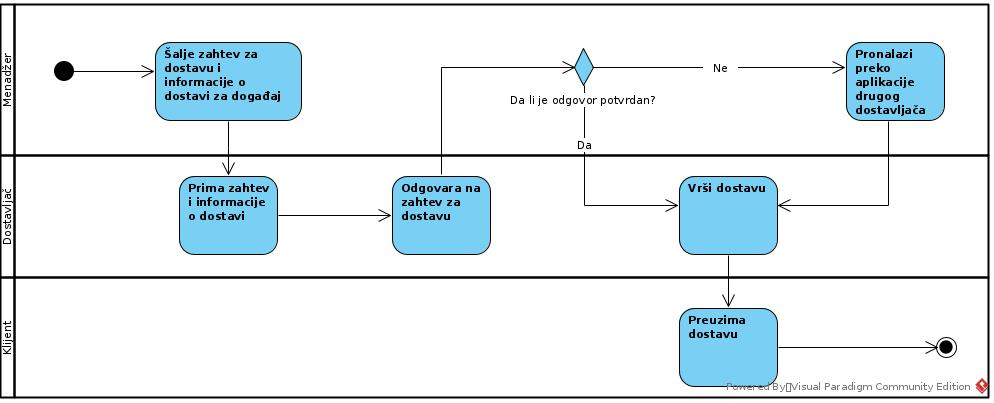
\includegraphics[width=15cm, height=8cm]{Milica/Dijagram_aktivnosti_Dostava_ketering.jpg}
    \caption{Dijagram aktivnosti Dostava keteringa}
    \label{fig:RegistracijaZ}
\end{figure}


%kraj-Milica
%%%%%%%%%%%%%%%%

\subsection{Naplata usluge}

\begin{figure}[H]
    \centering
    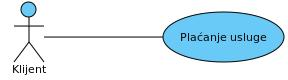
\includegraphics[width=6cm]{Nina/Slucaj_upotrebe_naplata.jpg}
    \caption{Dijagram slučaja upotrebe Naplata usluge}
    \label{fig:RegistracijaZ}
\end{figure}

\begin{itemize}
    \item Kratak opis: 
    \begin{itemize}
        \item Kada je usluga koju je klijent odabrao potpuno završena, on uplaćuje prethodno definisanu svotu novca preko sistema.
    \end{itemize}
    \item Učesnici:
        \begin{itemize}
        \item Klijent
    \end{itemize}
    \item Preduslov:
        \begin{itemize}
            \item Usluga koju je klijent izabrao je potpuno završena.
            \item Klijent ima otvoren nalog za korišćenje sistema.
        \end{itemize}
    \item Postuslov:
        \begin{itemize}
            \item Uplata je uspešno obavljena.
            \end{itemize}
    \item Glavni tok:
        \begin{enumerate}
            \item Klijent se prijavljuje na sistem firme Duma Group.
            \item Klikom na sekciju 'račun' klijent ima uvid u ukupnu cenu usluge, koja je bila ažurirana tokom vršenja usluge.
            \item Klijent klikom da dugme 'plaćanje' dobija formular koji popunjava podacima koji nedostaju kako bi izvršio uplatu.
            \item Klijent potvrđuje uplatu.
            \item Sistem vrši validaciju uplate.
            \item Sistem beleži uslugu kao uspešno regulisanu i čisti se sekcija 'račun' za klijenta.
        \end{enumerate}
    \item Alternativni tok:
        \begin{itemize}
            \item Korak 5 - Ukoliko uplata nije validna (broj računa je nepostojeći ili nije u dobrom formatu), sistem obaveštava korisnika o grešci i proces se nastavlja u koraku 4.  
    \end{itemize}
    \item Dodatne informacije:
        \begin{itemize}
            \item Podaci koje klijent treba da popuni su ime, prezime, adresa i broj žiro računa.
        \end{itemize}
\end{itemize}

\begin{figure}[H]
    \centering
    \includegraphics[width=8cm]{Nina/DIjagram_aktivnosti_naplata.jpg}
    \caption{Dijagram aktivnosti naplate usluge}
    \label{fig:RegistracijaZ}
\end{figure}

\end{document}
























